%
% newton.tex
%
% (c) 2020 Prof Dr Andreas Müller, Hochschule Rapperswil
%
\section{Newton-Verfahren
\label{buch:section:newtion}}
\rhead{Newton-Verfahren}
Die bisher vorgestellten Verfahren zur Bestimmung einer Nullstelle
$x^*$ der Funktion $f$, $f(x^*)=0$ sind eher langsam.
Dafür war nicht mehr als Stetigkeit nötig, um Konvergenz des Verfahrens
sicherzustellen.

\subsection{Analytischer Ansatz für ein quadratisch konvergentes Verfahren
\label{buch:subsection:newton:analytisch}}
In Abschnitt~\ref{buch:subsection:linearekonvergenz} wurde dargestellt,
dass nach Möglichkeit quadratische Konvergenz angestrebt werden sollte.
Quadratische Konvergenz könnte in einer Fixpunktiteration $x_{n+1}=g(x_n)$
erreicht werden, wenn die Ableitung $g'(x^*)=0$ ist.

Je grösser $f(x_n)$ ist, desto weiter dürfte $x_n$ von der Nullstelle
entfernt sein.
Wir versuchen daher, die Approximation $x_{n+}$ proportional zum Wert von
$f(x_n)$ zu korrigieren mit Hilfe der Funktion
\[
x_{n+1} = g(x_n) = x_n - a(x_n)\cdot f(x_n).
\]
Die Funktion $a(x_n)$ muss noch bestimmt werden.
Sie soll so gewählt werden, dass die Konvergenz quadratisch wird, was
mit $g'(x^*)=0$ erreicht wird.

Die Ableitung von $g$ ist
\begin{align*}
g'(x)
&=
1-a'(x)f(x)-a(x)f'(x).
\intertext{An der Stelle $x^*$ gilt}
g'(x^*)
&=
1-a'(x^*)\underbrace{f(x^*)}_{\displaystyle=0} - a(x^*)f'(x^*) = 0
\\
\Leftrightarrow\qquad
1
&=
a(x^*) f'(x^*)
\qquad\Rightarrow\qquad
a(x)=\frac{1}{f'(x)}.
\end{align*}
Damit finden wir das im folgenden Satz beschriebene Verfahren mit
quadratischer Konvergenz.

\begin{satz}[Newton-Verfahren]
\label{buch:satz:newton-verfahren}
Hat die differenzierbare Funktion $f$ eine Nullstelle $x^*$ und gilt
$f'(x^*)\ne 0$, dann konvergiert die Iterationsfolge
\begin{equation}
x_{n+1} = x_n - \frac{f(x_n)}{f'(x_n)} 
\label{buch:equation:newtoniteration}
\end{equation}
für Startwerte $x_0$ genügend nahe bei $x^*$ quadratisch gegen die
Nullstelle.
\end{satz}

\subsection{Geometrische Interpretation des Newton-Verfahrens}
\begin{figure}
\centering
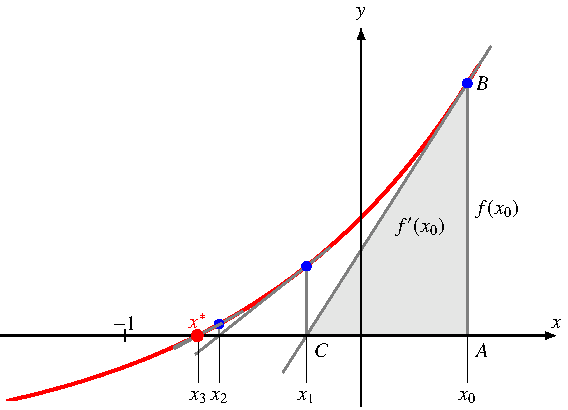
\includegraphics{chapters/20-gleichungen/figures/newton.pdf}
\caption{Graphische Interpretation des Newton-Verfahrens.
In jedem Iterationsschritt wird die bisherige Approximation $A$
mit Hilfe einer Tangente vom Funktionswert $B$ zum Punkt $C$
korrigiert, $\overline{AC}=f(x_0)/f'(x_0)$.
\label{buch:figure:newton}}
\end{figure}
Die Iterationsformel~\eqref{buch:equation:newtoniteration}
lässt sich sehr schön graphisch interpretieren.
In Abbildung~\ref{buch:figure:newton} wird die Nullstelle der
Funktion $f(x) = e^x-\frac12$ mit dem Newton-Verfahren bestimmt.
Im Iterationsschritt wird die Approximation $x_n$ korrigiert
nach der Formel
\[
x_{n+1}
=
x_n - \frac{f(x_n)}{f'(x_n)}
=
x_n - \frac{e^{x_n}-\frac12}{e^{x_n}}
=
x_n - \biggl(1 -\frac{e^{-x_n}}{2}\biggr)
\]
Die Korrektur für $n=0$ ist in Abbildung~\ref{buch:figure:newton}
als Grundseite des rechtwinkligen Dreiecks $ABC$ erkennbar.
Die Hypothenuse hat die Steigung $f'(x_0)$, daher ist
\[
\overline{AC}\cdot f'(x_0) = f(x_0)
\qquad\Rightarrow\qquad
\overline{AC} = \frac{f(x_0)}{f'(x_0)}.
\]
Die vom Newton-Verfahren berechnete Korrektur ist also die optimale
Korrektur, die sich berechnen lässt aus Funktionswert und erster Ableitung
an der Stelle $x_n$.

\subsection{Wurzeln}
Als Beispiel berechnen wir die $k$-te Wurzel einer positiven reellen
Zahl $a$, wir lösen also die Gleichung
$x^k = a$.
Dies ist gleichbedeutend damit, eine Nullstelle der Funktion
$f(x)=x^k-a$ zu bestimmen.
Die Ableitung von $f$ ist
$f'(x)=kx^{k-1}$, woraus wir die Iterationsformel des
Newton-Verfahrens ablesen können:
\[
x_{n+1} = x_n - \frac{f(x_n)}{f'(x_n)}=x_n - \frac{x_n^k-a}{kx_n^{k-1}}
=
\frac{1}{k}\biggl((k-1)x_n+\frac{a}{x_n^{k-1}}\biggr).
\]
Im Falle $n=2$ finden wir das bereits in 
Abschnitt~\ref{buch:subsection:linearekonvergenz}
untersuchte, quadratisch Konvergente Verfahren zur Bestimmung
der Quadratwurzel wieder.
In Tabelle~\ref{buch:table:wurzel5newton} ist das Verfahren für
$a=10$, $k=5$ und $x_0=a$ gezeigt.
Quadratische Konvergenz stellt sich allerdings erst bei $x_{10}$ ein,
der Startwert $x_0$ ist zu weit von der Lösung entfernt.

\begin{table}
\centering
\renewcommand\arraystretch{1.15}
\begin{tabular}{|>{$}r<{$}|>{$}r<{$}|}
\hline
n& x_n\\
\hline
 0 & 10.00000000000000\\
 1 &  8.00020000000000\\
 2 &  6.40064823242493\\
 3 &  5.12171019598693\\
 4 &  4.10027465454472\\
 5 &  3.28729556684556\\
 6 &  2.64696320430731\\
 7 &  2.15831219143923\\
 8 &  \underline{1}.81881622015378\\
 9 &  \underline{1.}63781027109793\\
10 &  \underline{1.58}820394873794\\
11 &  \underline{1.5849}0696686523\\
12 &  \underline{1.584893192}70054\\
13 &  \underline{1.58489319246111}\\
\hline
\infty&\sqrt[5]{10}=1.58489319246111\\
\hline
\end{tabular}
\caption{Berechnung von $\sqrt[5]{10}$ mit dem Newton-Verfahren.
Der Startwert $x_0=10$ ist sehr weit von der Lösung entfernt, so dass es
einige Iterationen braucht, bis die Konvergenz quadratisch wird.
\label{buch:table:wurzel5newton}}
\end{table}

\subsection{Newton-Verfahren in $\mathbb R^n$}
In der bisher beschriebenen Form erlaubt das Newton-Verfahren, 
Nullstellen von rellwertigen Funktion zu finden.
Es eignet sich nicht, Vektorgleichungen zu lösen.

Sei daher im folgenden $f\colon \mathbb R^n \to \mathbb R^n$ eine
Vektorfunktion mit einer Nullstelle $x^*$, $f(x^*)=0$, die numerisch gefunden 
werden soll.
Wie in Abschnitt~\ref{buch:subsection:newton:analytisch} soll eine
Approximation $x_n$ für die Nullstelle $x^*$ proportional zur Grösse
von $f(x_n)$ korrigiert werden.
Eine skalare Funktion $a(x)$ wird aber im allgemeinen zu wenig
allgemein für eine performante Lösung des Problem sein, daher
wird für $a(x)$ eine Funktion mit Werten in $\operatorname{GL}_2(\mathbb R)$
gewählt.
Wir setzen also an
\[
x_{n+1} = g(x_n) = x_n - a(x_n) f(x_n)
\]
und versuchen wie früher $a(x)$ so zu wählen, dass die Ableitung von $g$
an der Stelle $x^*$ verschwindet.

Die Ableitung von $g(x)=x-a(x)f(x)$ ist
\begin{align*}
Dg(x) \cdot h
&=
h - (Da(x)\cdot h) f(x) - a(x) Df(x)\cdot h.
\end{align*}
An der Stelle $x=x^*$ verschwindet der mittlere Term wegen $f(x^*)=0$, so
dass als Gleichung für $a(x)$
\[
0=h-a(x) Df(x) \cdot h
\qquad\Rightarrow\qquad
h = a(x) Df(x) \cdot h\qquad \forall h\in\mathbb R^n
\]
übrigbleibt.
Dies ist nur möglich, wenn $a(x)$ die inverse Matrix von $Df(x)$ ist,
was den folgenden Satz motiviert.

\begin{satz}[Newton-Verfahren für Vektorgleichungen]
Hat die Funktion $f\colon\mathbb R^n\to\mathbb R^n$ eine Nullstelle
$x^*\in\mathbb R^n$, dann ist die Folge 
\[
x_{n+1} = x_n - Df(x_n)^{-1}\cdot f(x_n)
\]
für Startwerte $x_0$ nahe genug an $x^*$ quadratisch konvergent mit
Grenzwert $x^*$.
\end{satz}

\begin{proof}[Beweis]
Es ist klar, das $x^*$ ein Fixpunkt der Abbildung
\[
g(x)=x-Df(x)^{-1}\cdot f(x)
\]
ist.
Wir müssen nur noch zeigen, dass der Fehler der Iteration quadratisch
abnimmt.
Dazu entwickeln wir $f$ um den Punkt ein eine Taylor-Reihe
\begin{align*}
f(x^* + \delta)
&=
f(x^*) + Df(x^*)\cdot \delta + O(|\delta|^2)
\\
&=
Df(x^*)\cdot \delta + O(|\delta|^2)
\end{align*}
wegen $f(x^*)=0$.
Die Iteration ist
\begin{align}
x_{n+1}
&=
x^* +\delta_{n+1}
=
g(x^*+\delta_n)
=
x^*+\delta_n  - Df(x_n)^{-1}\cdot f(x_n)
\notag
\\
&=
x^* + \delta_n -Df(x_n)^{-1}\cdot f(x^* + \delta_n)
\notag
\\
&=
x^* + \delta_n -Df(x_n)^{-1}\cdot
(Df(x^*)\cdot \delta_n + O(|\delta_n|^2).
\label{buch:equation:newtonn:iteration}
\end{align}
Um das zu berechnen, muss man auch $Df(x_n)$ noch entwickeln, es ist
\[
Df(x_n)
=
Df(x^*+\delta_n)
=
Df(x^*) + D^2f(x^*)\cdot\delta_n.
\]
Setzt man dies in~\eqref{buch:equation:newtonn:iteration} ein, erhält man
\begin{align*}
x_{n+1}
=
x^*+\delta_{n+1}
&=
x^* + \delta_n -
(Df(x^*) + D^2f(x^*)\cdot\delta_n)^{-1}
(Df(x^*)\cdot \delta_n + O(|\delta_n|^2)
\\
&=
x^* + \delta_n -
(Df(x^*)^{-1} + O(|\delta_n|))
\cdot
(Df(x^*)\cdot \delta_n + O(|\delta_n|^2)
\\
&=
x^* + \delta_n
- \underbrace{Df(x^*)^{-1}Df(x^*)}_{\displaystyle = E}\mathstrut\cdot\delta_n
+
O(|\delta_n|^2)
\\
&=x^* + O(|\delta_n|^2).
\end{align*}
Der Fehler $\delta_{n+1}=O(|\delta_n|^2)$ nimmt somit quadratisch ab
und damit ist gezeigt, dass die Iterationsfolge quadratrisch
konvergiert.
\end{proof}

\begin{beispiel}
Es sollen die Polarkoordinaten des Punktes $(x,y)$
als Lösung der Gleichung
\[
\begin{pmatrix}
r\cos\varphi\\r\sin\varphi
\end{pmatrix}
=
\begin{pmatrix}x\\y\end{pmatrix}
\qquad\Rightarrow\qquad
f(r,\varphi) =\begin{pmatrix}r\cos\varphi -x \\ r\sin\varphi -y \end{pmatrix}
=0
\]
bestimmt werden kann.

Die Ableitungsmatrix von $f$ ist
\[
Df(r,\varphi)
=
\begin{pmatrix}
\cos\varphi&-r \sin\varphi\\
\sin\varphi&\phantom{-} r \cos\varphi
\end{pmatrix}
\qquad\Rightarrow\qquad
Df(r,\varphi)^{-1}
=
\begin{pmatrix}
\cos\varphi&\sin\varphi\\
-\frac1r\sin\varphi&\frac1r\cos\varphi
\end{pmatrix}.
\]
Die Iterationsformel wird jetzt
\begin{align}
\begin{pmatrix}
r_{n+1}\\
\varphi_{n+1}
\end{pmatrix}
&=
\begin{pmatrix}r_n\\\varphi_n\end{pmatrix}
-
\begin{pmatrix}
\cos\varphi_n&\sin\varphi_n\\
-\frac1{r_n}\sin\varphi_n&\frac1{r_n}\cos\varphi_n
\end{pmatrix}
\begin{pmatrix}
r_n\cos\varphi_n-x\\
r_n\sin\varphi_n-y
\end{pmatrix}
\notag
\\
&=
\begin{pmatrix}
x\cos\varphi_n+y\sin\varphi_n\\
\varphi_n -\frac{x}{r_n}\sin\varphi_n+\frac{y}{r_n}\cos\varphi_n
\end{pmatrix}
\label{buch:equation:polar}
\end{align}
\begin{table}
\centering
\begin{tabular}{|>{$}r<{$}|>{$}r<{$}>{$}r<{$}|}
\hline
n &                r_n               &                    \varphi_n    \\
\hline
0 &              3.1415926535897931  &              0.3678794411714423 \\
1 &              0.8067763763745672  &              0.5559550343664228 \\
2 &   \underline{0.9}030213557712843 &   \underline{1.0}884392177149671 \\
3 &   \underline{0.99}60918007116625 &   \underline{0.99}06298199545209 \\
4 &   \underline{0.9999}561001841604 &   \underline{1.0000}366265580796 \\
5 &   \underline{0.999999999}3292477 &   \underline{0.99999999}83920385 \\
6 &   \underline{1.0000000000000000} &   \underline{1.0000000000000000} \\
\hline
\infty& 1.0000000000000000 &   1.0000000000000000 \\
\hline
\end{tabular}
\caption{Quadratische Konvergenz des Iterationsverfahrens
\eqref{buch:equation:polar}
zur Bestimmung der Polarkoordinaten 
\label{buch:figure:newtonpolar}}
\end{table}%
Die Resultate der Iteration~\eqref{buch:equation:polar} für 
den Punkt $(x,y)=(\cos 1,\sin 1)$ ist in 
Tabelle~\ref{buch:figure:newtonpolar} gegeben.
Die quadratische Konvergenz ist wieder deutlich erkennbar.
\end{beispiel}


